% To je predloga za poročila o domačih nalogah pri predmetih, katerih
% nosilec je Tomaž Curk. Avtor predloge je Blaž Zupan.
%
% Seveda lahko tudi dodaš kakšen nov, zanimiv in uporaben element,
% ki ga v tej predlogi (še) ni. Več o LaTeX-u izveš na
% spletu, na primer na http://tobi.oetiker.ch/lshort/lshort.pdf.%
% To predlogo lahko spremeniš v PDF dokument s pomočjo programa
% pdflatex, ki je del standardne instalacije LaTeX programov.

\documentclass[a4paper,11pt]{article}
\usepackage{a4wide}
\usepackage{fullpage}
\usepackage[utf8x]{inputenc}
\usepackage[english]{babel}
\selectlanguage{english}
\usepackage[toc,page]{appendix}
\usepackage[pdftex]{graphicx} % za slike
\usepackage{setspace}
\usepackage{color}
\definecolor{light-gray}{gray}{0.95}
\usepackage{listings}
\lstset{
  basicstyle=\ttfamily,
  columns=fullflexible,
  frame=single,
  breaklines=true,
  postbreak=\mbox{\textcolor{red}{$\hookrightarrow$}\space},
}
\usepackage{hyperref}
\renewcommand{\baselinestretch}{1.2} % za boljšo berljivost večji razmak
\renewcommand{\appendixpagename}{Appendix}

\lstset{ % nastavitve za izpis kode, sem lahko tudi kaj dodaš/spremeniš
language=Python,
basicstyle=\footnotesize,
basicstyle=\ttfamily\footnotesize\setstretch{1},
backgroundcolor=\color{light-gray},
}

\title{%
Analysis of song lyrics to match genre \\
\large Assignment 1: Basic text processing}
\author{Jernej Janež (63130077), Rok Marinšek (63130146), Luka Podgoršek (63130189)}
\date{\today}

\begin{document}

\maketitle

\section{NLP task}
% A paragraph of an NLP task/idea that you solved. A short description of your solution and related work in the field.
For our assignment we decided to analyze song lyrics, extract keywords that correspond to specific genres and try to classify song by its lyrics to corresponding genre. First we found a \href{https://www.kaggle.com/gyani95/380000-lyrics-from-metrolyrics}{\textit{dataset}} that contained song lyrics, then we preprocessed the data, trained and tested a model and presented results with tables and graphs. Some similar solutions already exist, but perform similar task with neural networks or some other more complex methods. With this assignment we wanted to find out if our approach can provide satisfactory results by using simple natural language processing techniques.

\section{Data}
% A description of (train, development, test) data or its retrieval
% Also describe metrics, used to score the performance of your algorithms.
We searched the internet for appropriate datasets and found many different ones but in the end decided to use \href{https://www.kaggle.com/gyani95/380000-lyrics-from-metrolyrics}{\textit{380,000+ lyrics from MetroLyrics dataset}} found on kaggle portal. This dataset had the attributes we needed to solve our task.

\noindent The dataset contained the following attributes:
\begin{itemize}
\item song title,
\item year,
\item artist
\item genre,
\item lyrics.
\end{itemize}

\subsection{Data preparation}
The data we found was stored in a \textit{.csv} file. Because it contained more than \textit{380 000} entries we decided to analyze songs that were released after year 2000 (latest songs in dataset). Afterwards we filtered the songs to match predefined genres which were \textit{hip-hop, pop and metal} and ended up with \textit{68244} different songs. Then we removed songs with lyrics that had less than 100 words and more than 1000 words which removed the outliers in the data.

When we finished preparing and selecting the data we focused on text preparation. First we removed special characters from text with regular expressions, converted words to lowercase and removed punctuations. Finally we removed non-english songs. This way we ended up with \textbf{5613} different songs.

\begin{table}[h!]
\centering
\label{baseline}
\begin{tabular}{|clc|}
\hline
\# & Genre & Number of different songs \\
\hline
0 & Hip-Hop & 20902 \\
1 & Metal & 16632 \\
2 & Pop & 30710 \\
\hline
\end{tabular}
\caption{Number of songs per genre}
\end{table}

In the end we saved the filtered data into a \textit{.csv} file and used it as input in our model class to train our model. You can also use this file to replicate our results.

\section{Model}

To train our model we used a preprocessed file and logistic regression.

\subsection{Train, test data and metrics}
% 80 20, regressing 0.2
% A description of (train, development, test) data or its retrieval. Also describe metrics, used to score the performance of your algorithms.
To train our model we used 80\% of data and 20\% to test our model. To measure score and performance of our model we used following metrics:
\begin{itemize}
\item accuracy,
\item precision,
\item recall,
\item and f1 score.
\end{itemize}

In development phase we also played with regularization factor. We used above mentioned metrics to determine the best regularization factor. In the end we set it to 0.1.

\subsection{Resources, tools and corpora}
%A description of tools and resources used. A list of additional linguistic corpora and how it was used to improve results of your algorithm

We used several different python libraries. Pandas was used for data structures and data purging. Nltk corpus was used to determine stopwords and for lemmatization. Langdetect library was used to remove non-english lyrics. To build our model we used sklearn and presented results with matplotlib.

\section{Algorithm-Model description}
% describe how we build our model

% we used l regression-.....

\subsection{Building bag of words with TF-IDF}
Bag of words is an algorithm that counts how many times a word appears in a document. We used WhitespaceTokenizer function from the ntlk library to tokenize our song lyrics and removed all the stop words, because words such as \textit{"and"} or \textit{"the"} appear frequently in all songs and are systematically discounted. Then we used the WordNetLemmatizer function also from the nltk library to lemmatize the text which grouped together the different inflected forms of a word so they can be analyzed as a single item. After that we vectorized our data with TF-IDF function called TfidfVectorizer from sklearn which measured the number of times words appeared in a given song (term frequency). The more songs a word appears in, the less valuable that word is as a signal. That’s intended to leave only the frequent AND distinctive words as markers. Each word’s TF-IDF relevance is a normalized data format that also adds up to one.


\section{Results}
% interpretacija modela, kaj je primerom skupno, zakaj pride do napačne klasifikacije

Before we could interpret our model and it's predictions we had to test it. Testing phase consisted of 10 iterations. In each iteration we sampled the data with different random seeds, trained a model and tested it on sampled test data. In the end we averaged all metrics to score the performance of our model. You can find the results in the \hyperref[label-model-score]{table} bellow.

\begin{table}[h!]
\centering
\label{baseline}
\begin{tabular}{|c|c|c|c|}
\hline
Accuracy & Precision & Recall & F1 \\
\hline
0.736 & 0.769 & 0.736 & 0.745 \\
\hline
\end{tabular}
\label{label-model-score}
\caption{Model scores}
\end{table}

\noindent Beside performance scores our model returned a list of keywords that have the most and the least value for classification. These results are presented in the tables bellow. Graphical presentation of tables is included in the appendix \hyperref[label-graphs]{graphs section.}

\begin{table}[h!]
\begin{tabular}{|lc|lc|}
\hline
(+) Keywords & Weight & (-) Keywords & Weight \\
\hline
death & 2.14 & love & -3.04 \\
blood & 1.95 & like & -2.23 \\
dead & 1.80 & oh & -2.10 \\
fucking & 1.68 & baby & -2.07 \\
end & 1.57 & girl & -2.01 \\
pain & 1.51 & i'm & -1.94 \\
hate & 1.48 & ain't & -1.93 \\
lie & 1.47 & yeah & -1.92 \\
die & 1.44 & got & -1.90 \\
fear & 1.42 & get & -1.61 \\
\hline
\end{tabular}
\quad
\begin{tabular}{|lc|lc|}
\hline
(+) Keywords & Weight & (-) Keywords & Weight \\
\hline
nigga & 3.90 & i've & -1.27 \\
shit & 2.72 & eye & -1.11 \\
ain't & 2.63 & lie & -1.07 \\
yo & 2.36 & dream & -0.96 \\
like & 2.32 & nothing & -0.86 \\
bitch & 2.24 & away & -0.83 \\
girl & 1.90 & heart & -0.80 \\
fuck & 1.75 & alone & -0.75 \\
cause & 1.74 & care & -0.73 \\
'em & 1.71 & world & -0.71 \\
\hline
\end{tabular}
\caption{Keywords for: \textbf{metal} (left) \& \textbf{hip-hop} (right)}
\end{table}

\begin{table}[h!]
\centering
\label{baseline}
\begin{tabular}{|lc|lc|}
\hline
(+) Keywords & Weight & (-) Keywords & Weight \\
\hline
love & 2.17 & nigga & -2.47 \\
oh & 1.85 & shit & -2.45 \\
heart & 1.58 & fuck & -2.21 \\
boy & 1.32 & death & -1.85 \\
gonna & 1.22 & fucking & -1.72 \\
baby & 1.06 & dead & -1.65 \\
blue & 1.05 & blood & -1.53 \\
'cause & 1.03 & bitch & -1.49 \\
could & 1.00 & die & -1.47 \\
kiss & 0.99 & hate & -1.40 \\
\hline
\end{tabular}
\caption{Keywords for \textbf{pop}}
\end{table}


%\begin{table}[h!]
%\centering
%\label{baseline}
%\begin{tabular}{cccc}
%\end{tabular}
%\caption{Keywords for hip-hop}
%\end{table}

\subsection{Postagging}
%top nouns and adjectives per genre

\begin{table}[h!]
\begin{tabular}{|lc|}
\hline

\hline
\end{tabular}
\quad
\begin{tabular}{|lc|lc|}
\hline

\hline
\end{tabular}
\caption{Nouns for: \textbf{metal} (left) \& \textbf{hip-hop} (right)}
\end{table}

\begin{table}[h!]
\centering
\label{baseline}
\begin{tabular}{|lc|}
\hline

\hline
\end{tabular}
\caption{Nouns for \textbf{pop}}
\end{table}

% slabosti modela
\subsection{Understanding wrong classifications}

If you look at our \hyperref[label-cf-matrix]{confusion matrix} you can notice that most commonly miss-classified songs are pop songs. We didn't expect to classify every song correctly, but pop songs have larger error rate than metal or hip-hop songs. We tried to understand why this was happening and our hypothesis was that many pop song artists feature artists from hip-hop or metal and therefore correlate with actual hip-hop and metal songs.

To test this we extracted songs that were not correctly classified. Afterwards we checked if song titles contained words \textit{"featuring"} or \textit{"ft"} or \textit{"feat"}. We counted the percentage of these songs and you can see results in the table bellow.


\section{Conclusion}


\section{Github repository}
Github repository: \href{https://github.com/marok39/onj-02}{https://github.com/marok39/onj-02}

\pagebreak
\appendix
\appendixpage
\section{\label{label-graphs} Graphs}

Here you can find the visualization of all results. These files can be found alongside the report in \textit{/img} directory.

\begin{figure}[h]
\begin{center}
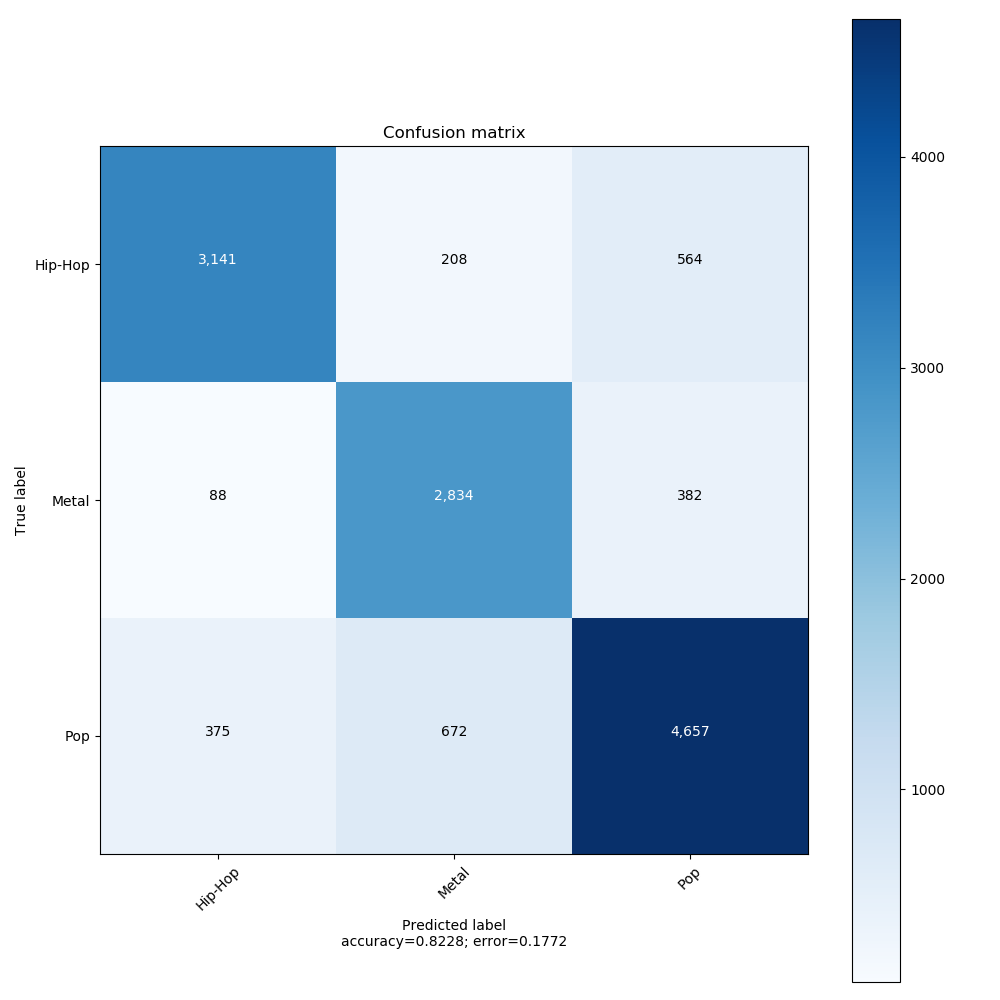
\includegraphics[width=0.8\textwidth]{./img/matrix.png}
\end{center}
\caption{Confusion matrix}
\label{label-cf-matrix}
\end{figure}

\begin{figure}[h]
\begin{center}
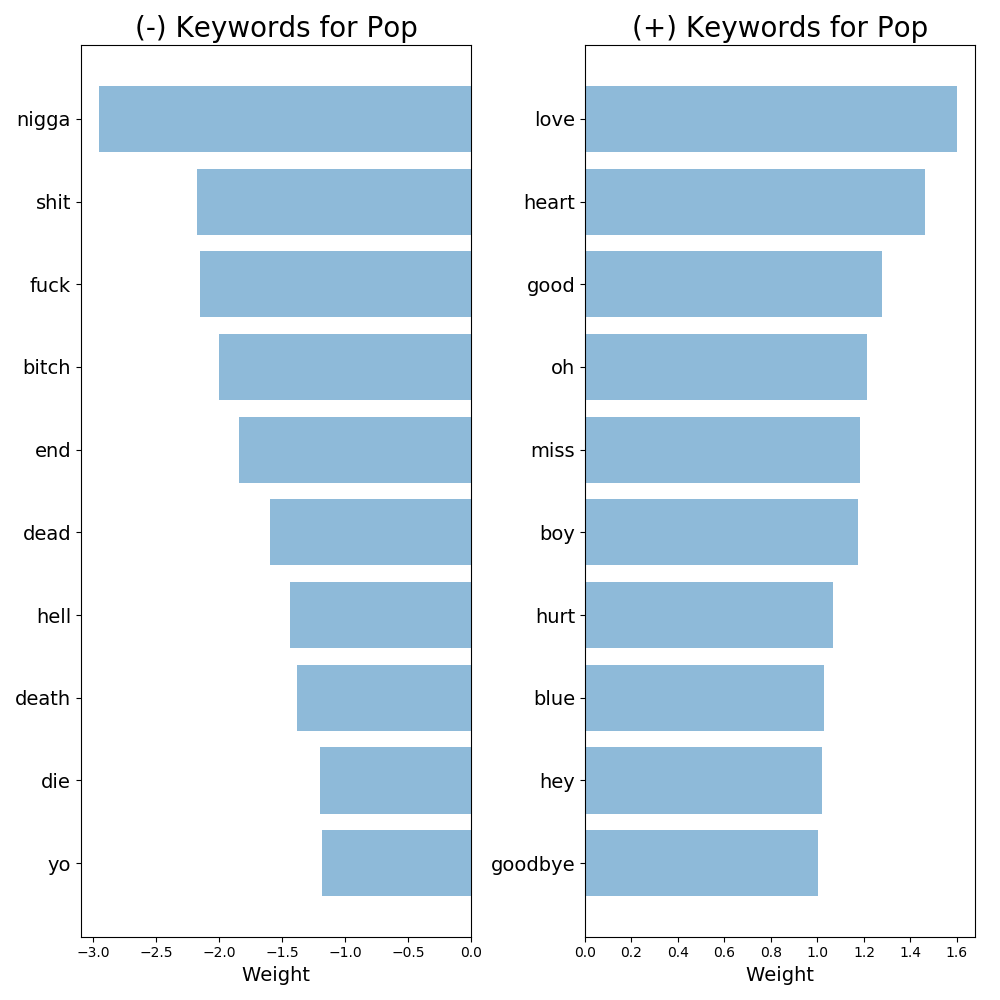
\includegraphics[width=0.8\textwidth]{./img/pop-keywords.png}
\end{center}
\caption{Keywords visualization for pop}
\label{label-kw-pop}
\end{figure}

\begin{figure}[h]
\begin{center}
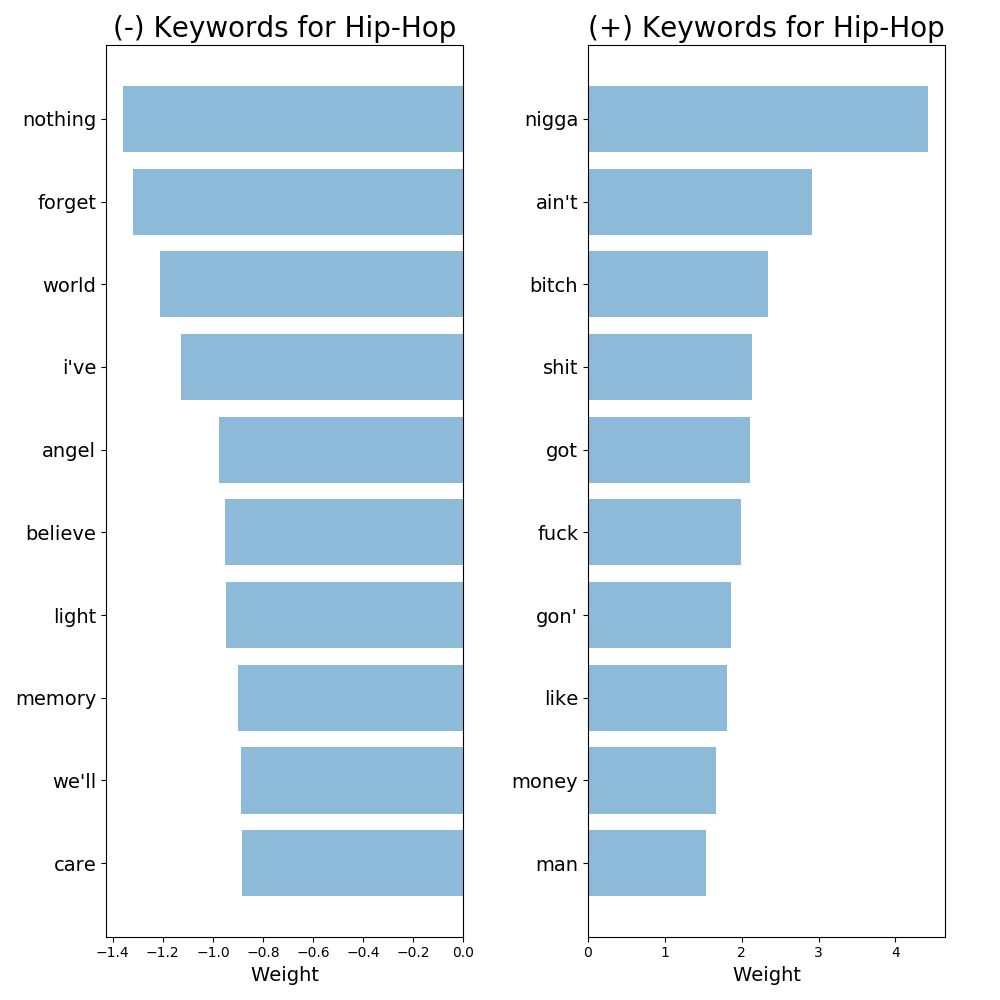
\includegraphics[width=0.8\textwidth]{./img/hip-hop-keywords.png}
\end{center}
\caption{Keywords visualization for hip-hop}
\label{label-kw-hip-hop}
\end{figure}

\begin{figure}[h]
\begin{center}
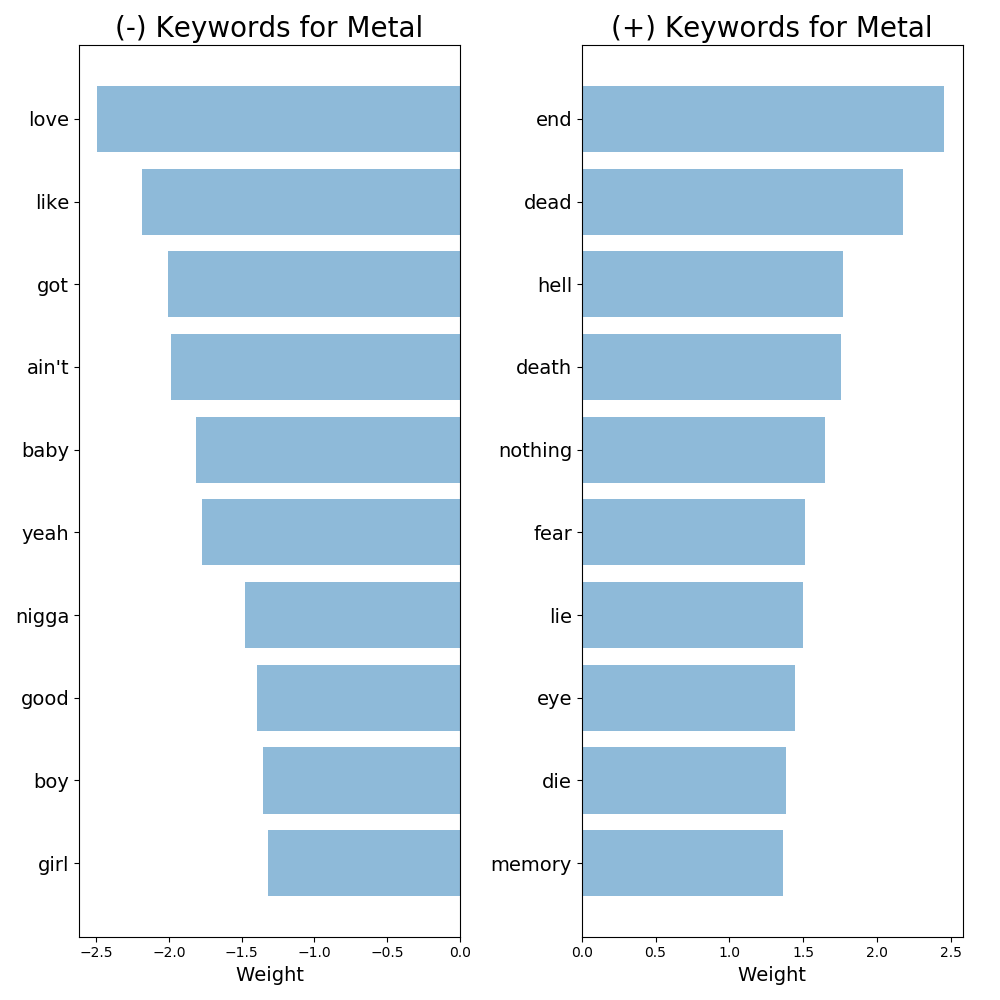
\includegraphics[width=0.8\textwidth]{./img/metal-keywords.png}
\end{center}
\caption{Keywords visualization for metal}
\label{label-kw-metal}
\end{figure}

%\begin{lstlisting}
%# comment
%\end{lstlisting}


\end{document}
